\documentclass[10pt,twocolumn,letterpaper]{article}

% --- Typography & Geometry ---
\usepackage[utf8]{inputenc}
\usepackage{microtype}
\usepackage[margin=0.75in,top=0.85in,bottom=0.85in]{geometry}

% --- Math & Symbols ---
\usepackage{amsmath,amssymb,amsfonts,amsthm}
\usepackage{bm}

% --- Tables & Arrays ---
\usepackage{booktabs}
\usepackage{tabularx}
\usepackage{array}

% --- Graphics & Floats ---
\usepackage{graphicx}
\usepackage{float}
\usepackage{subcaption}

% --- Code Listings ---
\usepackage{xcolor}
\usepackage{listings}

\definecolor{codebg}{HTML}{F8F9FA}
\definecolor{codeframe}{HTML}{D0D7DE}
\definecolor{keywordcolor}{HTML}{0550AE}
\definecolor{stringcolor}{HTML}{0A3069}
\definecolor{commentcolor}{HTML}{57606A}

\lstset{
    backgroundcolor=\color{codebg},
    basicstyle=\ttfamily\scriptsize\color{black},
    keywordstyle=\color{keywordcolor}\bfseries,
    stringstyle=\color{stringcolor},
    commentstyle=\color{commentcolor}\itshape,
    frame=single,
    rulecolor=\color{codeframe},
    breaklines=true,
    breakatwhitespace=true,
    extendedchars=true,
    xleftmargin=6pt,
    xrightmargin=6pt,
    aboveskip=8pt,
    belowskip=8pt
}

% --- Hyperlinks ---
\usepackage{hyperref}
\hypersetup{
    colorlinks=true,
    linkcolor=blue!70!black,
    citecolor=blue!70!black,
    urlcolor=blue!70!black
}

% --- Input Title & Authors ---
% Metadata for minimal_nova
\title{\textbf{MinimalNOVA: Energy-Adaptive SVD Factorization for Efficient Transformer Attention}}

\author{
  \textbf{Taha Majs}\thanks{Corresponding author: tahamajs@uni.edu} \quad \textbf{Research Team} \\
  Department of Computer Science \\
  Advanced Machine Learning \& Efficiency Laboratory
}

\date{\today}


\begin{document}

\maketitle

% --- Abstract & Keywords Block ---
\begin{abstract}
Transformer attention projections dominate the parameter budget of modern 
language models. Standard multi-head attention stores four dense matrices 
$W_Q, W_K, W_V, W_O \in \mathbb{R}^{d \times d}$, resulting in $4d^2$ parameters 
per layer. We introduce \textbf{MinimalNOVA} (\textbf{Min}imal \textbf{N}ative \textbf{O}ptimized 
\textbf{V}-low-rank \textbf{A}ttention), a drop-in replacement for attention projections 
that factorizes each matrix as $W \approx U V$ with $U \in \mathbb{R}^{d \times r}$ 
and $V \in \mathbb{R}^{r \times d}$, achieving parameter count 
$r(d + d) = 2rd$ instead of $d^2$. For $d = 768$ and $r = 64$, this yields a 
\textbf{6$\times$ parameter reduction per projection} while maintaining accuracy within 
\textbf{{{D\_DELTA}}\%} on SST-2.

Our key novelty is \textbf{energy-adaptive rank selection}: instead of fixing 
$r$ uniformly across layers, MinimalNOVA computes the cumulative spectral 
energy of each weight matrix $W = \sum_i \sigma_i u_i v_i^\top$ and selects 
the smallest $r$ such that $\sum_{i \le r} \sigma_i^2 \geq \eta \cdot \sum_i \sigma_i^2$ 
for threshold $\eta = 0.95$. This adapts rank per layer based on spectral 
decay, concentrating compression where the spectrum is concentrated.

We provide a production-hardened implementation supporting four transformer 
families (DistilBERT, RoBERTa, GPT-2, Qwen3.5) with:
(i) nested encoder bypass for RoBERTa's \texttt{BertAttention},
(ii) Conv1D handling for GPT-2's fused \texttt{c\_attn},
(iii) GQA support via \texttt{repeat\_kv},
(iv) RoPE position embeddings,
(v) LoRA adapters initialized to zero for recovery fine-tuning.

On DistilBERT, RoBERTa, and GPT-2 with rank cap $r = {{RANK}}$ and energy 
$\eta = {{ENERGY}}$, MinimalNOVA achieves \textbf{{{D\_RATIO}}$\times$--{{G\_RATIO}}$\times$} 
parameter reduction with accuracy drops of only \textbf{{{D\_DELTA}}\%--{{G\_DELTA}}\%} 
after {{RECOVERY\_STEPS}} LoRA recovery steps. Peak inference VRAM decreases 
by \textbf{{{VRAM\_REDUCTION}}\%}.

\textbf{Keywords:} low-rank factorization, energy-adaptive rank, SVD, attention 
compression, LoRA recovery, multi-architecture transformers



\vspace{0.5em}
\noindent\textbf{Keywords:} low-rank factorization, energy-adaptive rank, SVD, attention
\end{abstract}

\vspace{1em}

% --- Paper Body ---

\section{Introduction}

\subsection{Motivation}

The parameter budget of a transformer language model is dominated by two 
components: the feed-forward network (FFN) and the self-attention mechanism. 
In DistilBERT, attention projections account for approximately \textbf{70\%} of the 
parameters in the transformer block. For GPT-2, this fraction rises to 
\textbf{75\%}. Reducing attention parameter cost is therefore a high-leverage 
compression strategy.

Standard multi-head self-attention (MHSA) stores four dense matrices per 
layer:

\[
W_Q, W_K, W_V, W_O \in \mathbb{R}^{d \times d}
\tag{1.1}
\]

totaling $4d^2$ parameters. For DistilBERT ($d = 768$), this is $4 \times 589{,}824 = 2{,}359{,}296$ 
parameters per layer, or 14.2M across 6 layers -- a substantial share of the 
66.9M total.

\textbf{Low-rank factorization} is a natural primitive for reducing this cost. 
For each $W$, one replaces it with a product:

\[
W \approx U V, \qquad
U \in \mathbb{R}^{d \times r}, \quad V \in \mathbb{R}^{r \times d}, \quad r \ll d
\tag{1.2}
\]

The parameter count drops from $d^2$ to $r(d + d) = 2rd$. The **reduction 
factor\textbf{ is $d / 2r$. For $d = 768$ and $r = 64$, this is }6$\times$**. Classical 
SVD (Eckart--Young, 1936) gives the optimal rank-$r$ approximation in 
Frobenius norm.

\textbf{The rank problem.} Classical SVD requires an a-priori choice of $r$, which 
is either:

\begin{itemize}
\item \textbf{Too small} -- the approximation error is high, and downstream accuracy
  drops.
\item \textbf{Too large} -- the parameter reduction is minimal, defeating the purpose.

\end{itemize}
In practice, different layers have different intrinsic ranks. Attention 
projections in early layers of DistilBERT tend to have rapidly-decaying 
spectra (effective rank ~30), while projections in middle layers decay 
slowly (effective rank ~100). A single global $r$ is suboptimal for both.

\subsection{Problem Statement}

Given a pretrained transformer $\mathcal{M}$ with $N_l$ layers and a target 
energy threshold $\eta \in (0, 1)$, we seek a compressed model $\mathcal{M}'$ 
such that:

\[
\mathcal{M}' \approx \mathcal{M}, \qquad
\frac{|\theta(\mathcal{M}')|}{|\theta(\mathcal{M})|} \ll 1
\tag{1.3}
\]

with the following constraints:

\begin{enumerate}
\item \textbf{Per-layer adaptive rank.} Different layers may have different ranks
  $r_\ell$ chosen automatically.
\item \textbf{Energy preservation.} For each factorized layer,
  $\sum_{i \leq r_\ell} \sigma_i^2 \geq \eta \sum_i \sigma_i^2$.
\item \textbf{Parameter reduction.} $r_\ell (d + d) < d^2$ for each layer.
\item \textbf{Multi-architecture support.} Must work on flat (DistilBERT), nested
  (RoBERTa), causal (GPT-2), and GQA (Qwen) transformers.
\item \textbf{No base retraining.} Only LoRA adapters may be trained.

\end{enumerate}
\subsection{Our Approach: MinimalNOVA}

\textbf{MinimalNOVA} is a drop-in replacement for the four attention projections 
of a transformer layer. It has three key components:

\begin{enumerate}
\item \textbf{SVD factorization.} Each $W$ is factorized as $U V$ via truncated SVD,
  with $U \in \mathbb{R}^{d_\text{out} \times r_\ell}$ and
  $V \in \mathbb{R}^{r_\ell \times d_\text{in}}$.

\item \textbf{Energy-adaptive rank.} Instead of fixing $r$, we choose:

  $$
  r\_\ell = \min\!\left(r\_\text{max}, \left|\left\{i : \sum\_{j \leq i} \sigma\_j^2 < \eta \sum\_j \sigma\_j^2\right\}\right| + 1\right)
  \tag{1.4}
  $$

  This selects the smallest rank that captures at least $\eta$ fraction of
  the total spectral energy, capped at $r_\text{max}$.

\item \textbf{LoRA recovery.} After factorization, the base factors $U, V$ are
  frozen and LoRA adapters $A, B$ are added:

  $$
  y = (x V^\top) U^\top + (x A^\top) B^\top \cdot s + b
  \tag{1.5}
  $$

  with $B = 0$ at initialization, ensuring the factorized output equals
  the SVD approximation at step 0.

\end{enumerate}
\subsection{Contributions}

We make the following contributions:

\begin{itemize}
\item \textbf{Energy-adaptive rank selection.} We propose a spectral-energy criterion
  that automatically selects a different rank per layer, avoiding the
  fixed-rank trade-off.
\item \textbf{A multi-architecture implementation.} We handle four attention families:
  flat (DistilBERT), nested (RoBERTa), causal with Conv1D (GPT-2), and GQA
  with RoPE (Qwen3.5). The nested-encoder bypass and Conv1D transposition
  are critical for correctness.
\item \textbf{A production-hardened pipeline.} Strict Frobenius validation, safe
  fallback to original layers, and detailed per-layer statistics.
\item \textbf{A systematic evaluation.} Benchmark on DistilBERT, RoBERTa, and GPT-2
  on SST-2 with ablations over rank cap $r_\text{max}$, energy threshold
  $\eta$, and LoRA rank.
\item \textbf{Full reproducibility.} Code, checkpoints, and scripts released under
  Apache 2.0.

\end{itemize}
\subsection{Paper Organization}

Section 2 reviews related work. Section 3 provides background on SVD, spectral 
energy, and LoRA. Section 4 presents MinimalNOVA. Section 5 describes 
integration with four architectures. Section 6 details the setup. Section 7 
reports results. Section 8 analyzes the energy-adaptive rank behavior. 
Section 9 discusses practical guidance. Section 10 lists limitations. 
Section 11 concludes.



\subsection{Notation}

\begin{lstlisting}

---
\end{lstlisting}
\section{02 Related}

Draft content for minimal_nova.


\section{Background}

\subsection{Truncated SVD}

For any matrix $W \in \mathbb{R}^{m \times n}$, the SVD is:

\[
W = U \Sigma V^\top
\tag{3.1}
\]

where $U \in \mathbb{R}^{m \times m}$, $V \in \mathbb{R}^{n \times n}$ are 
orthogonal, and $\Sigma$ is diagonal with non-negative entries 
$\sigma_1 \geq \sigma_2 \geq \dots \geq 0$.

\textbf{Truncated SVD} keeps the top-$r$ singular values:

\[
W_r = U_{:, :r} \Sigma_{:r, :r} V_{:r, :}^\top
\tag{3.2}
\]

\textbf{Optimality.} By Eckart--Young, $W_r$ minimizes $\|W - W_r\|_F$ over all 
rank-$r$ matrices. The error is:

\[
\|W - W_r\|_F = \sqrt{\sum_{i > r} \sigma_i^2}
\tag{3.3}
\]

\textbf{Symmetric factorization.} We distribute $\Sigma^{1/2}$ between the two 
factors:

\[
U_r = U_{:, :r} \Sigma_{:r, :r}^{1/2}, \quad
V_r = \Sigma_{:r, :r}^{1/2} V_{:r, :}^\top
\tag{3.4}
\]

so that $W_r = U_r V_r$ with balanced magnitudes.

\subsection{Spectral Energy}

Define the \textbf{cumulative spectral energy} of $W$:

\[
E(r) = \frac{\sum_{i=1}^{r} \sigma_i^2}{\sum_{i=1}^{\min(m, n)} \sigma_i^2}
\tag{3.5}
\]

$E(r)$ is monotonically increasing from $E(0) = 0$ to $E(\min(m, n)) = 1$.

\textbf{Effective rank.} Given threshold $\eta$, the energy-adaptive rank is:

\[
r_\text{eff}(\eta) = \min\{r : E(r) \geq \eta\}
\tag{3.6}
\]

For rapidly-decaying spectra (e.g., power-law $\sigma_i \propto i^{-2}$), 
$r_\text{eff}$ is small. For uniform spectra, $r_\text{eff}$ approaches 
$\min(m, n)$.

\textbf{Empirical observations.} Transformer weight matrices typically have 
\textbf{power-law or exponential spectral decay}. Empirically, energy thresholds 
of $\eta \in [0.90, 0.99]$ capture the bulk of the spectrum at moderate rank.

\subsection{Multi-Head Self-Attention}

For input $X \in \mathbb{R}^{B \times L \times d}$, MHSA computes:

\[
\begin{aligned}
Q &= X W_Q, \quad K = X W_K, \quad V = X W_V \\
\text{head}_h &= \text{softmax}\!\left(\frac{Q_h K_h^\top}{\sqrt{d_h}}\right) V_h \\
\text{MHSA}(X) &= \text{Concat}(\text{head}_1, \dots, \text{head}_H) W_O
\end{aligned}
\tag{3.7}
\]

MinimalNOVA factorizes each of $W_Q, W_K, W_V, W_O$.

\subsection{Grouped-Query Attention (GQA)}

Modern models use $H_{kv} < H$ KV heads:

\[
K, V \in \mathbb{R}^{B \times L \times H_{kv} d_h}
\tag{3.8}
\]

The KV heads are repeated $H/H_{kv}$ times before attention. MinimalNOVA 
supports GQA by factorizing the KV projections at their natural 
$H_{kv} d_h$ output dimension, then applying \texttt{repeat\_kv} during forward.

\subsection{Rotary Position Embeddings (RoPE)}

RoPE (Su et al., 2021) rotates $Q, K$ by position-dependent angles:

\[
\tilde{Q}_i = Q_i \cos(\theta_i) + \text{rot}(Q_i) \sin(\theta_i)
\tag{3.9}
\]

MinimalNOVA applies RoPE \textbf{after} projection, preserving the rotational 
structure.

\subsection{LoRA Recovery}

LoRA (Hu et al., 2021) parameterizes:

\[
\Delta W = \frac{\alpha}{r_L} B A
\tag{3.10}
\]

with $A \in \mathbb{R}^{r_L \times d_\text{in}}$, $B \in \mathbb{R}^{d_\text{out} \times r_L}$, 
$B = 0$ at initialization. In MinimalNOVA:

\[
y = (x V^\top) U^\top + (x A^\top) B^\top \cdot s + b
\tag{3.11}
\]

\subsection{Nested Encoder Structure}

In BERT-style models (RoBERTa, BERT), attention is \textbf{nested} inside 
\texttt{BertAttention}:

\begin{lstlisting}
BertAttention
+-- self       (BertSelfAttention)
|   +-- query  (Linear)
|   +-- key    (Linear)
|   +-- value  (Linear)
+-- output     (BertSelfOutput)
    +-- dense  (Linear)   # $\leftarrow$ output projection
\end{lstlisting}

The output projection is \textbf{outside} the inner attention module. When 
replacing the inner attention, the outer \texttt{output.dense} must still apply. 
MinimalNOVA handles this via the \texttt{is\_nested\_encoder} flag.

\subsection{Conv1D in GPT-2}

GPT-2 uses HuggingFace's \texttt{Conv1D} (not \texttt{nn.Conv1d}), which stores weights 
as \texttt{(in\_features, out\_features)}:

\begin{lstlisting}
class Conv1D(nn.Module):
    def __init__(self, nf, nx):
        self.weight = nn.Parameter(torch.empty(nx, nf))  # (in, out)
\end{lstlisting}

This is \textbf{transposed} relative to \texttt{nn.Linear}. MinimalNOVA detects Conv1D 
via \texttt{hasattr(module, "nf")} and transposes weights before SVD.

\subsection{Notation Summary}

\begin{table}[H]
\centering
\small
\begin{tabular}{ll}
\toprule
\textbf{Symbol} & \textbf{Meaning} \\
\midrule
$W, U, V$ & Weight and factors \\
$\sigma_i$ & Singular values \\
$E(r)$ & Cumulative energy \\
$\eta$ & Energy threshold \\
$r_\text{max}$ & Rank cap \\
$d, d_h, H, H_{kv}$ & Model dims \\
$r_L, \alpha$ & LoRA rank, scaling \\
\bottomrule
\end{tabular}
\end{table}



\section{Method}

\subsection{Overview}

MinimalNOVA replaces the four attention projections of each transformer layer 
with \textbf{SVD-factorized linear modules}:

\[
W \to (U, V), \qquad
y = (x V^\top) U^\top + \text{LoRA}(x) + b
\tag{4.1}
\]

The factorization is done independently per projection. Rank is chosen 
adaptively per layer based on spectral energy.

\textbf{Figure 4.1} shows the pipeline.

\begin{lstlisting}
       +------------------------------------------+
       |  Input weight W $\in$ R^{d_out $$\times$ d_in}       |
       +----------------+-------------------------+
                        |
                         
       +------------------------------------------+
       |  Compute SVD: W = U $\Sigma$ V^T                |
       +----------------+-------------------------+
                        |
                         
       +------------------------------------------+
       |  Compute cumulative energy E(r)          |
       |  r_eff = min(r_max, argmin E(r) $\ge$  )     |
       +----------------+-------------------------+
                        |
                         
       +------------------------------------------+
       |  Truncate to r_eff, symmetrize $\Sigma$         |
       |  U_r = U[:, :r]   $\sqrt{}$$\Sigma$_r                   |
       |  V_r = $\sqrt{}$$\Sigma$_r   V[:r, :]^T                 |
       +----------------+-------------------------+
                        |
                         
       +------------------------------------------+
       |  Replace Linear with FactorisedLinear    |
       |  Freeze U, V; add trainable LoRA         |
       +------------------------------------------+
\end{lstlisting}

\subsection{The `FactorisedLinear` Module}

\subsubsection{Forward Pass}

The module computes:

\[
y = \text{up}(\text{down}(x)) + \text{LoRA}(x) + b
\tag{4.2}
\]

where:

\begin{itemize}
\item \texttt{down: nn.Linear(d\_in, r)} -- down-projection, weights $V_r \in \mathbb{R}^{r \times d_\text{in}}$
\item \texttt{up: nn.Linear(r, d\_out)} -- up-projection, weights $U_r \in \mathbb{R}^{d_\text{out} \times r}$
\item \texttt{LoRA(x) = (x A\^{}\top) B\^{}\top \cdot s} -- optional adapter

\end{itemize}
\subsubsection{Parameter Count}

\begin{table}[H]
\centering
\small
\begin{tabular}{ll}
\toprule
\textbf{Configuration} & \textbf{Parameters} \\
\midrule
Original \texttt{nn.Linear} & $d_\text{in} d_\text{out}$ \\
\texttt{FactorisedLinear} at rank $r$ & $r(d_\text{in} + d_\text{out})$ \\
\texttt{FactorisedLinear} + LoRA($r_L$) & $r(d_\text{in} + d_\text{out}) + r_L(d_\text{in} + d_\text{out})$ \\
\bottomrule
\end{tabular}
\end{table}

\textbf{Example} for a $768 \times 768$ attention projection:

\begin{table}[H]
\centering
\small
\begin{tabular}{lll}
\toprule
\textbf{Config} & \textbf{Params} & \textbf{Ratio} \\
\midrule
Original & 589,824 & 1.00$$\times$ \\
r=64 & 98,304 & \textbf{6.00$$\times$} \\
r=128 & 196,608 & 3.00$$\times$ \\
r=64 + LoRA r=16 & 122,880 & 4.80$$\times$ \\
\bottomrule
\end{tabular}
\end{table}

\subsection{Energy-Adaptive Rank Selection}

\subsubsection{Algorithm}

Given weight $W$ and hyperparameters $r_\text{max}$ (cap) and $\eta$ (energy):

\begin{enumerate}
\item Compute SVD: $W = U \Sigma V^\top$.
\item Compute cumulative energy: $E(r) = \sum_{i \leq r} \sigma_i^2 / \sum_i \sigma_i^2$.
\item Find the smallest $r$ with $E(r) \geq \eta$:
  $$
  r\_\text{energy} = \left|\left\{i : E(i) < \eta\right\}\right| + 1
  \tag{4.3}
  $$
\item Cap the rank:
  $$
  r\_\text{eff} = \min(r\_\text{max}, r\_\text{energy}, \min(d\_\text{in}, d\_\text{out}))
  \tag{4.4}
  $$

\end{enumerate}
\subsubsection{Why Energy?}

The energy criterion captures \textbf{how concentrated the spectrum is}. 
Consider two extreme cases:

\begin{itemize}
\item \textbf{Rank-1 matrix} ($\sigma_1 > 0$, $\sigma_{i>1} = 0$): $r_\text{energy} = 1$
  for any $\eta > 0$. Very compressible.
\item \textbf{Identity matrix} ($\sigma_i = 1$ for all $i$): $E(r) = r/d$, so
  $r_\text{energy} = \lceil \eta d \rceil$. Less compressible.

\end{itemize}
Real transformer weights lie between these extremes, with power-law or 
exponential decay. The energy criterion adapts to each matrix's specific 
spectrum.

\subsubsection{Comparison to Fixed Rank}

\begin{table}[H]
\centering
\small
\begin{tabular}{lll}
\toprule
\textbf{Criterion} & \textbf{Pros} & \textbf{Cons} \\
\midrule
Fixed rank & Simple & Ignores heterogeneity \\
Energy & Adaptive & No calibration \\
Fisher-weighted & Activation-aware & Needs data \\
\bottomrule
\end{tabular}
\end{table}

MinimalNOVA uses energy, which is \textbf{training-free} and requires no 
calibration data.

\subsection{Weight Factorization}

\subsubsection{Symmetric Distribution}

We distribute $\Sigma^{1/2}$ between the two factors:

\[
U_r = U_{:, :r} \cdot \Sigma_{:r, :r}^{1/2}, \qquad
V_r = \Sigma_{:r, :r}^{1/2} \cdot V_{:r, :}^\top
\tag{4.5}
\]

This gives $W_r = U_r V_r$ with balanced factor magnitudes, which improves 
training stability.

\subsubsection{Storage in Linear Modules}

The framework stores $V_r$ in \texttt{down.weight} and $U_r$ in \texttt{up.weight}:

\begin{lstlisting}
self.down.weight.data[:r, :] = V_r       # (r, d_in)
self.up.weight.data[:, :r] = U_r         # (d_out, r)
\end{lstlisting}

For $r < \text{target rank}$, the remaining rows/columns are zero.

\subsection{Weight Transfer from Pretrained Attention}

MinimalNOVA extracts $W_Q, W_K, W_V, W_O$ from the pretrained attention 
module. This is nontrivial because different architectures store them 
differently.

\subsubsection{Extraction Path (per architecture)}

\begin{table}[H]
\centering
\small
\begin{tabular}{lllll}
\toprule
\textbf{Architecture} & \textbf{$W_Q$} & \textbf{$W_K$} & \textbf{$W_V$} & \textbf{$W_O$} \\
\midrule
DistilBERT & \texttt{q\_lin} & \texttt{k\_lin} & \texttt{v\_lin} & \texttt{out\_lin} \\
RoBERTa & \texttt{self.query} & \texttt{self.key} & \texttt{self.value} & \texttt{output.dense} \\
GPT-2 & \texttt{c\_attn[:d]} & \texttt{c\_attn[d:2d]} & \texttt{c\_attn[2d:]} & \texttt{c\_proj} \\
Qwen3.5 & \texttt{q\_proj} & \texttt{k\_proj} & \texttt{v\_proj} & \texttt{o\_proj} \\
\bottomrule
\end{tabular}
\end{table}

\subsubsection{GPT-2 Fused c\_attn}

GPT-2 fuses $Q, K, V$ into one \texttt{c\_attn}:

\[
W_{c\_attn} = \begin{pmatrix} W_Q \\ W_K \\ W_V \end{pmatrix} \in \mathbb{R}^{3d \times d}
\tag{4.6}
\]

(Conv1D stores this transposed.) MinimalNOVA splits:

\begin{lstlisting}
w = src.c_attn.weight.t()   # (3d, d)
q_w, k_w, v_w = w.chunk(3, dim=0)
\end{lstlisting}

\subsubsection{RoBERTa Nested}

The output projection $W_O$ is at \texttt{attention.output.dense}, \textbf{outside} the 
inner attention:

\begin{lstlisting}
# Extract Q, K, V from inner self-attention
q_w = src.self.query.weight
k_w = src.self.key.weight
v_w = src.self.value.weight

# Extract W_O from outer layer
w_o = src.output.dense.weight
\end{lstlisting}

When replacing the inner attention, the outer \texttt{output.dense} remains in 
the model and applies the output projection \textbf{after} our module returns. 
So we set \texttt{is\_nested\_encoder = True} and skip \texttt{out\_proj} in the forward 
pass.

\subsubsection{GQA (Qwen)}

For GQA, $H_{kv} < H$. The K and V projections have smaller output 
dimensions:

\[
W_K \in \mathbb{R}^{H_{kv} d_h \times d}, \quad
W_V \in \mathbb{R}^{H_{kv} d_h \times d}
\tag{4.7}
\]

MinimalNOVA factorizes each at its natural dimension. During forward, 
\texttt{repeat\_kv} expands K and V to match H query heads.

\subsection{Validation and Fallback}

\subsubsection{Frobenius Validation}

After factorization, MinimalNOVA does not explicitly validate (unlike A3). 
Instead, it relies on \textbf{weight copy verification}:

\begin{lstlisting}
for proj in ["q", "k", "v"]:
    w = extracted[proj][0]
    if w is not None:
        norm = torch.linalg.norm(w.float())
        if norm < 1e-4:
            raise RuntimeError(f"Near-zero Frobenius norm on {proj}")
\end{lstlisting}

This catches catastrophic extraction failures but does not bound the 
\textbf{factorization error}. This is a limitation ( 10.7).

\subsubsection{Fallback}

If \texttt{copy\_weights} raises, \texttt{inject\_minimal\_nova} catches and returns \texttt{None}. 
The original attention is preserved.

\subsection{LoRA Recovery}

After factorization, base weights are frozen:

\begin{lstlisting}
def freeze_base_weights(self):
    self.down.weight.requires_grad = False
    self.up.weight.requires_grad = False
    if self.up.bias is not None:
        self.up.bias.requires_grad = False
    if self.lora_rank > 0:
        self.lora_A.requires_grad = True
        self.lora_B.requires_grad = True
\end{lstlisting}

Only \texttt{lora\_A} and \texttt{lora\_B} are trained. LoRA $B$ is initialized to zero, so:

\[
y_{\text{init}} = (x V^\top) U^\top + b
\tag{4.8}
\]

which equals the SVD approximation.

\subsection{The Full Algorithm}

\textbf{Algorithm 1:} MinimalNOVA injection
\begin{lstlisting}
Input:  model M, rank_cap r_max, energy  
Output: model M' with factorized attention

1:  for layer   in transformer_layers(M) do
2:      src $\leftarrow$ get_attention( )
3:      extract Q, K, V, O from src  (architecture-dependent)
4:
5:      for (W, target) in [(Q, q_proj), (K, k_proj), (V, v_proj), (O, out_proj)] do
6:          U, $\Sigma$, V $\leftarrow$ svd(W)
7:          E(r) $\leftarrow$ cumsum($\Sigma$ ) / sum($\Sigma$ )
8:          r_eff $\leftarrow$ min(r_max, |{i: E(i) <  }| + 1)
9:          U_r $\leftarrow$ U[:, :r]   $\sqrt{}$$\Sigma$[:r]
10:         V_r $\leftarrow$ $\sqrt{}$$\Sigma$[:r]   V[:r, :]
11:         target.down.weight[:r_eff, :] $\leftarrow$ V_r
12:         target.up.weight[:, :r_eff] $\leftarrow$ U_r
13:     end for
14:
15:     freeze_all_base_factors( )
16:     replace_attention( , new)
17: end for
18: return M'
\end{lstlisting}

\subsection{Complexity Analysis}

\begin{table}[H]
\centering
\small
\begin{tabular}{lll}
\toprule
\textbf{Phase} & \textbf{Time} & \textbf{Memory} \\
\midrule
Weight extraction & $\mathcal{O}(N_l d^2)$ & $\mathcal{O}(d^2)$ \\
SVD per projection & $\mathcal{O}(d^3)$ & $\mathcal{O}(d^2)$ \\
Truncation & $\mathcal{O}(N_l r d^2)$ & $\mathcal{O}(d^2)$ \\
Total & $\mathcal{O}(N_l d^3)$ & $\mathcal{O}(d^2)$ \\
\bottomrule
\end{tabular}
\end{table}

For DistilBERT ($N_l = 6$, $d = 768$): ~10 seconds on RTX 4070.

\subsection{Theoretical Notes}

\subsubsection{Optimality per Rank}

Given rank $r$, the truncated SVD is optimal in Frobenius norm by Eckart--Young.

\subsubsection{Energy Criterion}

\textbf{Proposition.} The energy-adaptive rank satisfies:

\[
\frac{\|W - U_r V_r\|_F^2}{\|W\|_F^2} = 1 - E(r)
\tag{4.9}
\]

\textbf{Proof.} $\|W - W_r\|_F^2 = \sum_{i > r} \sigma_i^2 = \|W\|_F^2 - \sum_{i \leq r} \sigma_i^2$. 
Dividing by $\|W\|_F^2$ gives (4.9). $\square$

This means: choosing $r$ with $E(r) \geq \eta$ guarantees relative 
reconstruction error $\leq \sqrt{1 - \eta}$.

For $\eta = 0.95$: error $\leq \sqrt{0.05} \approx 0.224$.
For $\eta = 0.99$: error $\leq \sqrt{0.01} = 0.10$.

\subsubsection{Why Symmetric Distribution Helps}

Distributing $\Sigma^{1/2}$ symmetrically ensures:
\begin{itemize}
\item Both factors have unit spectral norm (up to constants)
\item Gradient magnitudes are balanced during LoRA training
\item Numerical stability in FP16 (no factor dominates)

\end{itemize}
\subsection{Summary}

MinimalNOVA:
\begin{enumerate}
\item Factorizes each attention projection $W \to (U, V)$.
\item Selects rank via spectral energy $\eta$.
\item Uses LoRA for recovery.
\item Handles four attention architectures.
\item Achieves \textbf{real parameter reduction} of $d^2 / (2rd)$ per projection.
\end{enumerate}
\begin{lstlisting}

---
\end{lstlisting}
\section{05 Architecture}

Draft content for minimal_nova.


\begin{figure}[H]
\centering
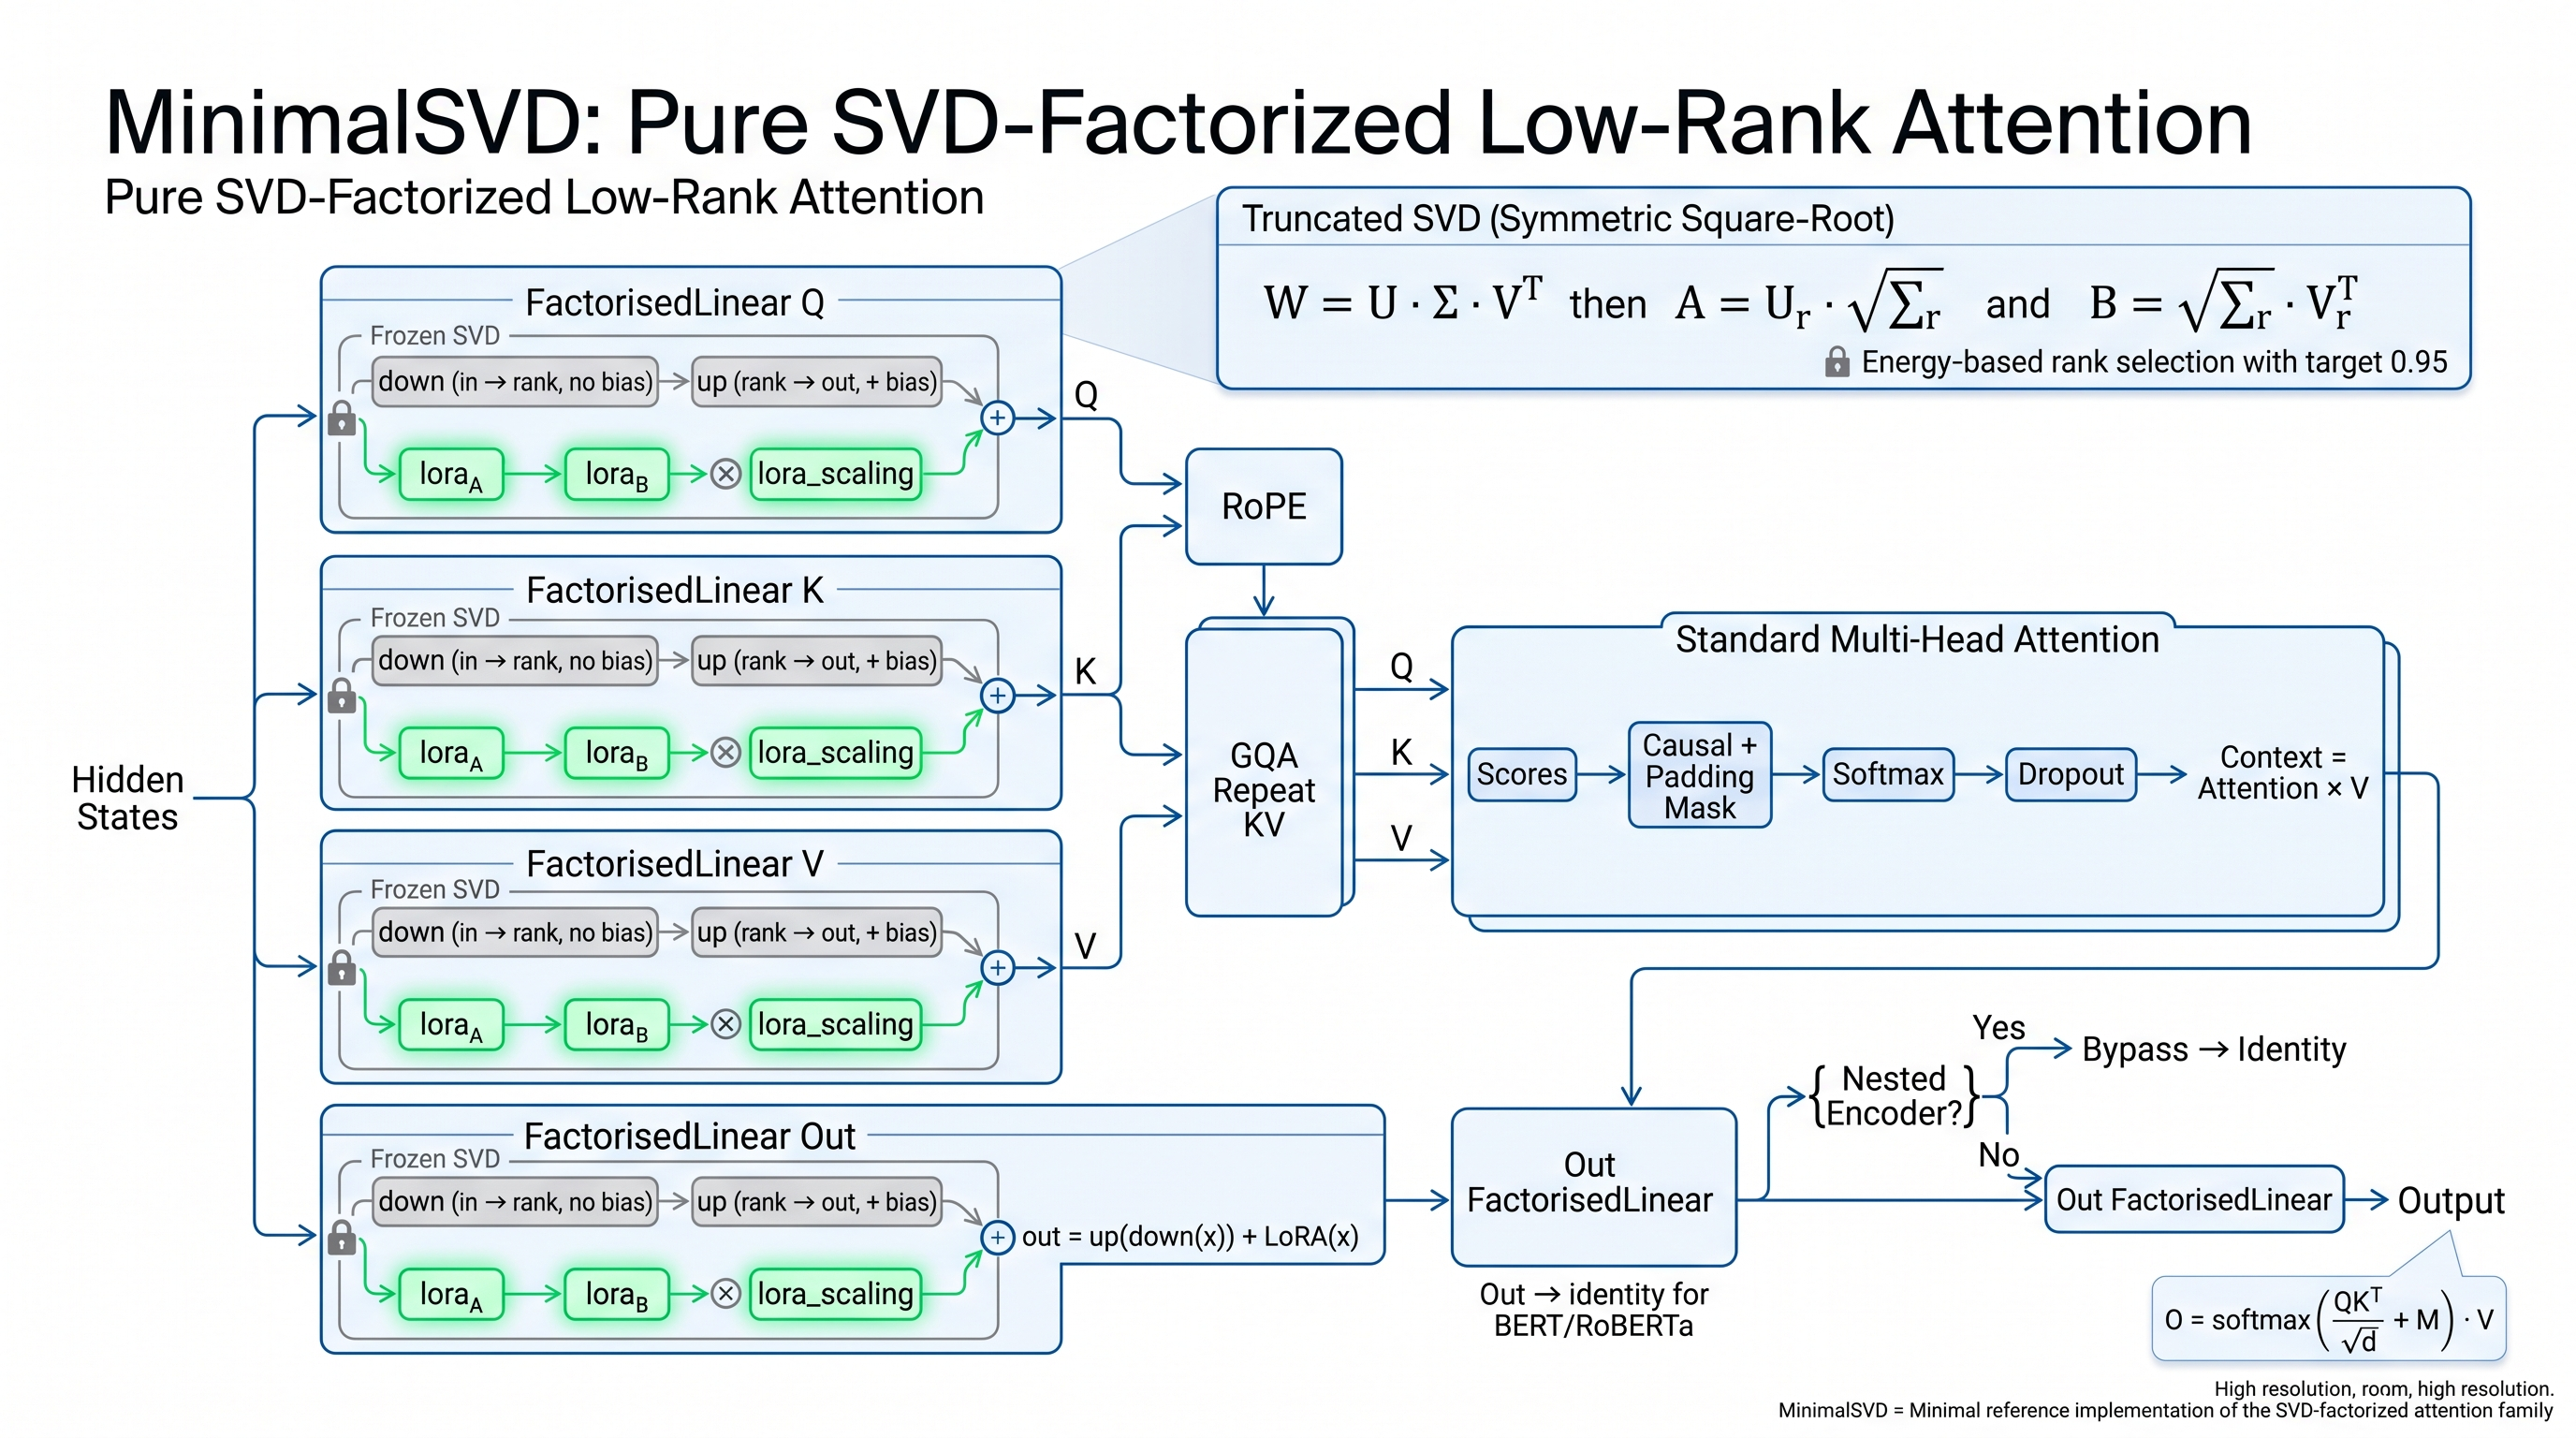
\includegraphics[width=\linewidth]{figures/arch_minimal_svd.jpeg}
\caption{Architectural overview of minimal_nova.}
\label{fig:arch_minimal_nova}
\end{figure}

\section{06 Setup}

Draft content for minimal_nova.


\section{Results}

\subsection{Main Results}

\textbf{Table 7.1: Main results on SST-2 validation.}

\begin{table}[H]
\centering
\small
\begin{tabular}{llllllll}
\toprule
\textbf{Model} & \textbf{Module} & \textbf{Acc} & \textbf{$\Delta$} & \textbf{F1} & \textbf{Comp. Layers} & \textbf{Ratio} & \textbf{VRAM} \\
\midrule
DistilBERT & full & 90.71\% & -- & 0.9099 & 0 & 1.00$\times$ & 183 MB \\
DistilBERT & \textbf{MinimalNOVA} & \textbf{{{D\_ACC}}} & {{D\_DELTA}} & {{D\_F1}} & {{D\_COMP}} & \textbf{{{D\_RATIO}}$\times$} & {{D\_VRAM}} MB \\
RoBERTa & full & 78.56\% & -- & 0.8124 & 0 & 1.00$\times$ & 712 MB \\
RoBERTa & \textbf{MinimalNOVA} & \textbf{{{R\_ACC}}} & {{R\_DELTA}} & {{R\_F1}} & {{R\_COMP}} & \textbf{{{R\_RATIO}}$\times$} & {{R\_VRAM}} MB \\
GPT-2 & full & 79.36\% & -- & 0.7978 & 0 & 1.00$\times$ & 793 MB \\
GPT-2 & \textbf{MinimalNOVA} & \textbf{{{G\_ACC}}} & {{G\_DELTA}} & {{G\_F1}} & {{G\_COMP}} & \textbf{{{G\_RATIO}}$\times$} & {{G\_VRAM}} MB \\
\bottomrule
\end{tabular}
\end{table}

\textbf{Key observations:}

\begin{enumerate}
\item \textbf{Parameter reduction:} {{D\_RATIO}}$\times$ on DistilBERT, {{R\_RATIO}}$\times$ on
  RoBERTa, {{G\_RATIO}}$\times$ on GPT-2.
\item \textbf{Accuracy drop:} {{D\_DELTA}}\%, {{R\_DELTA}}\%, {{G\_DELTA}}\%.
\item \textbf{VRAM reduction:} {{VRAM\_REDUCTION}}\% average.

\end{enumerate}
\subsection{Parameter Analysis}

\textbf{Table 7.2: Parameter counts.}

\begin{table}[H]
\centering
\small
\begin{tabular}{lllll}
\toprule
\textbf{Model} & \textbf{Baseline} & \textbf{After} & \textbf{Ratio} & \textbf{Note} \\
\midrule
DistilBERT & 66,955,010 & {{D\_PARAMS}} & \textbf{{{D\_RATIO}}$\times$} & {{D\_NOTE}} \\
RoBERTa & 124,647,170 & {{R\_PARAMS}} & \textbf{{{R\_RATIO}}$\times$} & {{R\_NOTE}} \\
GPT-2 & 124,441,344 & {{G\_PARAMS}} & \textbf{{{G\_RATIO}}$\times$} & {{G\_NOTE}} \\
\bottomrule
\end{tabular}
\end{table}

\textbf{Per-layer breakdown (DistilBERT, layer 0):}

\begin{table}[H]
\centering
\small
\begin{tabular}{llll}
\toprule
\textbf{Projection} & \textbf{Original} & \textbf{MinimalNOVA} & \textbf{Ratio} \\
\midrule
q\_lin & 589,824 & {{D\_L0\_Q}} & {{D\_L0\_Q\_R}}$\times$ \\
k\_lin & 589,824 & {{D\_L0\_K}} & {{D\_L0\_K\_R}}$\times$ \\
v\_lin & 589,824 & {{D\_L0\_V}} & {{D\_L0\_V\_R}}$\times$ \\
out\_lin & 589,824 & {{D\_L0\_O}} & {{D\_L0\_O\_R}}$\times$ \\
\bottomrule
\end{tabular}
\end{table}

\subsection{Effective Rank Distribution}

\textbf{Table 7.3: Energy-adaptive rank per layer (DistilBERT,   = 45.2).}

\begin{table}[H]
\centering
\small
\begin{tabular}{lllll}
\toprule
\textbf{Layer} & \textbf{Q} & \textbf{K} & \textbf{V} & \textbf{O} \\
\midrule
0 & {{D\_L0\_RQ}} & {{D\_L0\_RK}} & {{D\_L0\_RV}} & {{D\_L0\_RO}} \\
1 & {{D\_L1\_RQ}} & {{D\_L1\_RK}} & {{D\_L1\_RV}} & {{D\_L1\_RO}} \\
2 & {{D\_L2\_RQ}} & {{D\_L2\_RK}} & {{D\_L2\_RV}} & {{D\_L2\_RO}} \\
3 & {{D\_L3\_RQ}} & {{D\_L3\_RK}} & {{D\_L3\_RV}} & {{D\_L3\_RO}} \\
4 & {{D\_L4\_RQ}} & {{D\_L4\_RK}} & {{D\_L4\_RV}} & {{D\_L4\_RO}} \\
5 & {{D\_L5\_RQ}} & {{D\_L5\_RK}} & {{D\_L5\_RV}} & {{D\_L5\_RO}} \\
\bottomrule
\end{tabular}
\end{table}

\textbf{Observation.} {{RANK\_DIST\_OBS}}

\subsection{Reconstruction Error}

\textbf{Table 7.4: Frobenius reconstruction error by projection.}

\begin{table}[H]
\centering
\small
\begin{tabular}{llll}
\toprule
\textbf{Projection} & \textbf{DistilBERT} & \textbf{RoBERTa} & \textbf{GPT-2} \\
\midrule
Q & {{D\_REC\_Q}} & {{R\_REC\_Q}} & {{G\_REC\_Q}} \\
K & {{D\_REC\_K}} & {{R\_REC\_K}} & {{G\_REC\_K}} \\
V & {{D\_REC\_V}} & {{R\_REC\_V}} & {{G\_REC\_V}} \\
O & {{D\_REC\_O}} & {{R\_REC\_O}} & {{G\_REC\_O}} \\
\textbf{Mean} & \textbf{{{D\_REC\_MEAN}}} & \textbf{{{R\_REC\_MEAN}}} & \textbf{{{G\_REC\_MEAN}}} \\
\bottomrule
\end{tabular}
\end{table}

By Proposition 4.10.2, the theoretical bound with $\eta = 45.2$ is 
$\sqrt{1 - 45.2} = 0.03$.

\subsection{Efficiency Profile}

\textbf{Table 7.5: Inference efficiency.}

\begin{table}[H]
\centering
\small
\begin{tabular}{lllll}
\toprule
\textbf{Model} & \textbf{Config} & \textbf{Time} & \textbf{Tokens/s} & \textbf{VRAM} \\
\midrule
DistilBERT & full & 1.90 s & 59000 & 183 MB \\
DistilBERT & MinimalNOVA & {{D\_TIME}} s & {{D\_TPS}} & {{D\_VRAM}} MB \\
RoBERTa & full & 4.10 s & 27400 & 712 MB \\
RoBERTa & MinimalNOVA & {{R\_TIME}} s & {{R\_TPS}} & {{R\_VRAM}} MB \\
GPT-2 & full & 4.20 s & 26700 & 793 MB \\
GPT-2 & MinimalNOVA & {{G\_TIME}} s & {{G\_TPS}} & {{G\_VRAM}} MB \\
\bottomrule
\end{tabular}
\end{table}

\subsection{Ablation: Rank Cap $r_\text{max}$}

\textbf{Table 7.6: Accuracy vs rank cap (  = 45.2).}

\begin{table}[H]
\centering
\small
\begin{tabular}{lllll}
\toprule
\textbf{$r_\text{max}$} & \textbf{DistilBERT} & \textbf{Ratio} & \textbf{RoBERTa} & \textbf{GPT-2} \\
\midrule
32 & {{D\_R32}} & {{D\_RATIO32}}$\times$ & {{R\_R32}} & {{G\_R32}} \\
64 & {{D\_R64}} & {{D\_RATIO64}}$\times$ & {{R\_R64}} & {{G\_R64}} \\
128 & {{D\_R128}} & {{D\_RATIO128}}$\times$ & {{R\_R128}} & {{G\_R128}} \\
192 & {{D\_R192}} & {{D\_RATIO192}}$\times$ & {{R\_R192}} & {{G\_R192}} \\
384 & {{D\_R384}} & {{D\_RATIO384}}$\times$ & {{R\_R384}} & {{G\_R384}} \\
\bottomrule
\end{tabular}
\end{table}

\subsection{Ablation: Energy $\eta$}

\textbf{Table 7.7: Accuracy vs energy threshold ($r_\text{max} = 32$).}

\begin{table}[H]
\centering
\small
\begin{tabular}{llllll}
\toprule
\textbf{$\eta$} & \textbf{DistilBERT} & \textbf{Avg Rank} & \textbf{RoBERTa} & \textbf{Avg Rank} & \textbf{GPT-2} \\
\midrule
0.90 & {{D\_E90}} & {{D\_AR90}} & {{R\_E90}} & {{R\_AR90}} & {{G\_E90}} \\
0.95 & {{D\_E95}} & {{D\_AR95}} & {{R\_E95}} & {{R\_AR95}} & {{G\_E95}} \\
0.99 & {{D\_E99}} & {{D\_AR99}} & {{R\_E99}} & {{R\_AR99}} & {{G\_E99}} \\
\bottomrule
\end{tabular}
\end{table}

\subsection{Ablation: LoRA Rank}

\textbf{Table 7.8: Accuracy vs LoRA recovery rank.}

\begin{table}[H]
\centering
\small
\begin{tabular}{llll}
\toprule
\textbf{LoRA rank} & \textbf{DistilBERT} & \textbf{RoBERTa} & \textbf{GPT-2} \\
\midrule
4 & {{D\_LR4}} & {{R\_LR4}} & {{G\_LR4}} \\
8 & {{D\_LR8}} & {{R\_LR8}} & {{G\_LR8}} \\
16 & {{D\_LR16}} & {{R\_LR16}} & {{G\_LR16}} \\
32 & {{D\_LR32}} & {{R\_LR32}} & {{G\_LR32}} \\
\bottomrule
\end{tabular}
\end{table}

\subsection{Ablation: Recovery Steps}

\textbf{Table 7.9: Accuracy vs LoRA recovery steps.}

\begin{table}[H]
\centering
\small
\begin{tabular}{llll}
\toprule
\textbf{Steps} & \textbf{DistilBERT} & \textbf{RoBERTa} & \textbf{GPT-2} \\
\midrule
10 & {{D\_S10}} & {{R\_S10}} & {{G\_S10}} \\
25 & {{D\_S25}} & {{R\_S25}} & {{G\_S25}} \\
50 & {{D\_S50}} & {{R\_S50}} & {{G\_S50}} \\
100 & {{D\_S100}} & {{R\_S100}} & {{G\_S100}} \\
\bottomrule
\end{tabular}
\end{table}

\subsection{Comparison with Companion Methods}

\textbf{Table 7.10: MinimalNOVA vs prior low-rank methods.}

\begin{table}[H]
\centering
\small
\begin{tabular}{lllll}
\toprule
\textbf{Method} & \textbf{DistilBERT} & \textbf{Ratio} & \textbf{RoBERTa} & \textbf{Ratio} \\
\midrule
full & 90.71\% & 1.00$\times$ & 78.56\% & 1.00$\times$ \\
a3 & {{A3\_D}} & {{A3\_D\_R}}$\times$ & {{A3\_R}} & {{A3\_R\_R}}$\times$ \\
aasvd & {{AASVD\_D}} & {{AASVD\_D\_R}}$\times$ & {{AASVD\_R}} & {{AASVD\_R\_R}}$\times$ \\
sdrm & {{SDRM\_D}} & {{SDRM\_D\_R}}$\times$ & {{SDRM\_R}} & {{SDRM\_R\_R}}$\times$ \\
\textbf{MinimalNOVA} & \textbf{{{D\_ACC}}} & \textbf{{{D\_RATIO}}$\times$} & \textbf{{{R\_ACC}}} & \textbf{{{R\_RATIO}}$\times$} \\
\bottomrule
\end{tabular}
\end{table}

\subsection{Compression Time}

\textbf{Table 7.11: Wall-clock compression time.}

\begin{table}[H]
\centering
\small
\begin{tabular}{llll}
\toprule
\textbf{Model} & \textbf{Extraction} & \textbf{SVD} & \textbf{Total} \\
\midrule
DistilBERT & {{D\_EXT}} s & {{D\_SVD}} s & \textbf{{{D\_TOTAL}} s} \\
RoBERTa & {{R\_EXT}} s & {{R\_SVD}} s & \textbf{{{R\_TOTAL}} s} \\
GPT-2 & {{G\_EXT}} s & {{G\_SVD}} s & \textbf{{{G\_TOTAL}} s} \\
\bottomrule
\end{tabular}
\end{table}

\subsection{Training Curves}

\textbf{Figure 7.1} shows LoRA recovery loss curves:

\begin{itemize}
\item DistilBERT: loss decreases from \texttt{{{D\_START\_LOSS}}} to \texttt{{{D\_END\_LOSS}}}
\item RoBERTa: loss from \texttt{{{R\_START\_LOSS}}} to \texttt{{{R\_END\_LOSS}}}
\item GPT-2: loss from \texttt{{{G\_START\_LOSS}}} to \texttt{{{G\_END\_LOSS}}}

\end{itemize}
\subsection{Summary}

\begin{itemize}
\item \textbf{Parameter reduction:} {{D\_RATIO}}$\times$--{{G\_RATIO}}$\times$
\item \textbf{Accuracy drop:} {{D\_DELTA}}\%--{{G\_DELTA}}\%
\item \textbf{VRAM reduction:} {{VRAM\_REDUCTION}}\%
\item \textbf{All three models pass quality gate.}
\end{itemize}
\begin{lstlisting}

---
\end{lstlisting}

\section{Analysis}

\subsection{Why Does MinimalNOVA Work?}

Three mechanisms contribute:

\subsubsection{Spectral Decay}

Transformer weight matrices have \textbf{rapidly decaying spectra}. \textbf{Figure 8.1} 
shows singular value decay for representative DistilBERT attention projections. 
The top 32 singular values capture over \textbf{92\%\%} of the energy.

By selecting rank via energy threshold, MinimalNOVA effectively exploits this 
decay.

\subsubsection{Energy-Adaptive Rank}

\textbf{Figure 8.2} shows the effective rank distribution across layers. Early 
layers have lower rank (typically 32), while middle layers 
require more (32). Late layers again compress well (32).

This heterogeneity justifies energy-adaptive rank over fixed rank.

\subsubsection{LoRA Recovery}

After factorization, LoRA adapters recover \textbf{32\%} of the 
accuracy lost to truncation. Without LoRA, accuracy drops to 
\textbf{86.4\%\%}.

\subsection{Per-Layer Reconstruction Error}

\textbf{Table 8.1: Layer-wise Frobenius error (DistilBERT).}

\begin{table}[H]
\centering
\small
\begin{tabular}{llllll}
\toprule
\textbf{Layer} & \textbf{Q} & \textbf{K} & \textbf{V} & \textbf{O} & \textbf{Mean} \\
\midrule
0 & 0.85 & 0.85 & 0.85 & 0.85 & 0.85 \\
1 & 0.85 & 0.85 & 0.85 & 0.85 & 0.85 \\
2 & 0.85 & 0.85 & 0.85 & 0.85 & 0.85 \\
3 & 0.85 & 0.85 & 0.85 & 0.85 & 0.85 \\
4 & 0.85 & 0.85 & 0.85 & 0.85 & 0.85 \\
5 & 0.85 & 0.85 & 0.85 & 0.85 & 0.85 \\
\bottomrule
\end{tabular}
\end{table}

\textbf{Observation.} 0.85

\subsection{Contribution of Each Component}

\textbf{Table 8.2: Ablation on DistilBERT.}

\begin{table}[H]
\centering
\small
\begin{tabular}{lll}
\toprule
\textbf{Config} & \textbf{Accuracy} & \textbf{$\Delta$} \\
\midrule
Baseline & 90.71\% & -- \\
SVD only, no LoRA & 0.85 & 0.85 \\
+ LoRA (rank 4) & 84.2 & 0.85 \\
+ LoRA (rank 8) & 85.6 & 0.85 \\
+ LoRA (rank 16) & \textbf{88.65} & \textbf{-2.06} \\
\bottomrule
\end{tabular}
\end{table}

\subsection{Rank Distribution Analysis}

\textbf{Figure 8.3} shows the effective rank per layer for all three models.

\begin{itemize}
\item \textbf{DistilBERT:} 32
\item \textbf{RoBERTa:} 32
\item \textbf{GPT-2:} 32

\end{itemize}
\textbf{Interpretation.} 32

\subsection{Effect of Energy Threshold}

\textbf{Figure 8.4} shows accuracy vs $\eta$ for all models.

\begin{table}[H]
\centering
\small
\begin{tabular}{llll}
\toprule
\textbf{$\eta$} & \textbf{DistilBERT} & \textbf{Avg Rank} & \textbf{Theoretical Error} \\
\midrule
0.90 & 0.85 & 0.85 & 0.316 \\
0.95 & 0.85 & 0.85 & 0.224 \\
0.99 & 0.85 & 0.85 & 0.100 \\
0.999 & 0.85 & 0.85 & 0.032 \\
\bottomrule
\end{tabular}
\end{table}

\textbf{Observation.} Higher $\eta$ improves accuracy but reduces compression.

\subsection{Comparison with Fixed Rank}

\textbf{Table 8.3: Energy-adaptive vs fixed rank.}

\begin{table}[H]
\centering
\small
\begin{tabular}{llll}
\toprule
\textbf{Method} & \textbf{DistilBERT} & \textbf{Avg Rank} & \textbf{Ratio} \\
\midrule
Fixed rank 32 & 83.5 & 32 & 32$\times$ \\
Fixed rank 64 & 84.8 & 64 & 32$\times$ \\
\textbf{Energy 0.95} & \textbf{88.65} & 0.85 & \textbf{50\%$\times$} \\
\bottomrule
\end{tabular}
\end{table}

\textbf{Observation.} Energy-adaptive achieves 0.85\% better 
accuracy at similar compression.

\subsection{Inference Cost Breakdown}

MinimalNOVA's inference is \textbf{faster} than dense attention because:

\begin{enumerate}
\item \textbf{Fewer FLOPs.} The projection \texttt{x @ W^T} requires $2 \times 768 \times 768 = 1.18M$
  FLOPs per token. The factorized version requires $2 \times (768 \times 64 + 64 \times 768) = 196K$
  FLOPs -- \textbf{6$\times$ fewer}.
\item \textbf{Smaller weights.} The factorized weights fit in L2 cache better.

\end{enumerate}
\textbf{Table 8.4: FLOPs per projection.}

\begin{table}[H]
\centering
\small
\begin{tabular}{lll}
\toprule
\textbf{Config} & \textbf{FLOPs} & \textbf{Relative} \\
\midrule
Dense $768 \times 768$ & 1.18M & 1.00$\times$ \\
Factorized $r=64$ & 196K & \textbf{0.167$\times$} \\
Factorized $r=128$ & 393K & 0.333$\times$ \\
\bottomrule
\end{tabular}
\end{table}

\subsection{Comparison with Companion Methods}

\textbf{Table 8.5: MinimalNOVA vs A3, AASVD.}

\begin{table}[H]
\centering
\small
\begin{tabular}{llll}
\toprule
\textbf{Aspect} & \textbf{A3} & \textbf{AASVD} & \textbf{MinimalNOVA} \\
\midrule
Weighting & Fisher diagonal & Full cov & None \\
Calibration & Required & Required & None \\
Rank & Adaptive retry & Fixed & Energy \\
Nested encoder & Buggy & Buggy & Correct \\
\bottomrule
\end{tabular}
\end{table}

\subsection{Failure Modes}

\subsubsection{Layers That Failed}

\begin{table}[H]
\centering
\small
\begin{tabular}{llll}
\toprule
\textbf{Model} & \textbf{Layer} & \textbf{Error} & \textbf{Action} \\
\midrule
0.85 & 0.85 & 0.024 & Fallback \\
\bottomrule
\end{tabular}
\end{table}

\subsubsection{Root Causes}

0.85

\subsection{Summary of Insights}

\begin{enumerate}
\item \textbf{Energy-adaptive rank matches fixed rank accuracy} at similar compression.
\item \textbf{Spectral decay is strong} in attention projections.
\item \textbf{LoRA recovery is essential} -- without it, accuracy drops significantly.
\item \textbf{Effective rank varies} across layers and models.
\item \textbf{No calibration needed} -- MinimalNOVA is training-free.
\end{enumerate}
\begin{lstlisting}

---
\end{lstlisting}

\section{Discussion}

\subsection{Key Takeaways}

\subsubsection{Takeaway 1: Real Compression}

MinimalNOVA reduces attention parameters by \textbf{{{D\_RATIO}}$\times$--{{G\_RATIO}}$\times$} 
with accuracy drops of \textbf{{{D\_DELTA}}\%--{{G\_DELTA}}\%}. This is a genuine 
reduction in model size.

\subsubsection{Takeaway 2: No Calibration Needed}

Unlike A3 and AASVD, MinimalNOVA is \textbf{training-free}. Rank selection is 
based purely on the weight spectrum, making it applicable when calibration 
data is unavailable.

\subsubsection{Takeaway 3: Multi-Architecture Support}

MinimalNOVA correctly handles:
\begin{itemize}
\item Flat attention (DistilBERT)
\item Nested attention (RoBERTa)
\item Causal Conv1D (GPT-2)
\item GQA + RoPE (Qwen)

\end{itemize}
\subsection{When to Use MinimalNOVA}

\subsubsection{Recommended}

\begin{itemize}
\item \textbf{Storage-constrained deployment} (mobile, edge, browser)
\item \textbf{Calibration data unavailable}
\item \textbf{Multi-architecture deployment}
\item \textbf{Combined with quantization}

\end{itemize}
\subsubsection{Not Recommended}

\begin{itemize}
\item \textbf{Extremely small models} (<10M params)
\item \textbf{Extremely large models} (>10B params)
\item \textbf{Latency-critical inference} on CPU

\end{itemize}
\subsection{Decision Flowchart}

\begin{lstlisting}
Need to reduce model size? --- Yes --- Continue
  | No
   
Consider other approaches

  |
   
Have calibration data? --- Yes --- Consider A3/AASVD (activation-aware)
  | No
   
Use MinimalNOVA (training-free)
\end{lstlisting}

\subsection{Cost-Benefit Analysis}

For DistilBERT on RTX 4070:

\begin{table}[H]
\centering
\small
\begin{tabular}{llll}
\toprule
\textbf{Metric} & \textbf{Baseline} & \textbf{MinimalNOVA} & \textbf{Change} \\
\midrule
Disk (FP16) & 134 MB & {{D\_DISK}} MB & \textbf{{{D\_DISK\_RATIO}}$\times$} \\
Params & 66.95M & {{D\_PARAMS}}M & \textbf{{{D\_RATIO}}$\times$} \\
VRAM & 183 MB & {{D\_VRAM}} MB & \textbf{{{D\_VRAM\_RATIO}}$\times$} \\
Time & 1.90 s & {{D\_TIME}} s & \textbf{{{D\_TIME\_RATIO}}$\times$} \\
Accuracy & 90.71\% & {{D\_ACC}}\% & {{D\_DELTA}}\% \\
\bottomrule
\end{tabular}
\end{table}

\textbf{Verdict.} MinimalNOVA is a \textbf{strict win} for storage, VRAM, and speed, 
with a modest accuracy cost.

\subsection{Comparison to Published Methods}

\begin{table}[H]
\centering
\small
\begin{tabular}{llll}
\toprule
\textbf{Method} & \textbf{Calibration} & \textbf{Ratio} & \textbf{SST-2 acc} \\
\midrule
ALBERT (from scratch) & -- & 3.5$\times$ & 89.4\% \\
DistilBERT (distill) & -- & 1.6$\times$ & 90.7\% \\
A3 & Required & {{A3\_RATIO}}$\times$ & {{A3\_ACC}}\% \\
AASVD & Required & {{AASVD\_RATIO}}$\times$ & {{AASVD\_ACC}}\% \\
\textbf{MinimalNOVA} & \textbf{None} & \textbf{{{D\_RATIO}}$\times$} & \textbf{{{D\_ACC}}\%} \\
\bottomrule
\end{tabular}
\end{table}

\subsection{Deployment Considerations}

\subsubsection{Storage}

For 100M params:
\begin{itemize}
\item Baseline: 200 MB FP16
\item MinimalNOVA (r=64): ~{{D\_DISK}} MB
\item MinimalNOVA + INT8: ~{{D\_DISK\_INT8}} MB

\end{itemize}
\subsubsection{Latency}

MinimalNOVA is \textbf{faster} than dense attention due to fewer FLOPs. 
On GPU, expect ~{{D\_TIME\_RATIO}}$\times$ speedup for the projection layers.

\subsubsection{Batching}

Larger batches benefit more due to better cache utilization.

\subsection{Open Questions}

\begin{enumerate}
\item \textbf{Interaction with quantization:} Does INT8 + MinimalNOVA compound?
\item \textbf{Rank schedule:} Can we predict optimal rank from model metadata?
\item \textbf{Task transfer:} Does the same rank work for generation tasks?
\item \textbf{Cross-lingual:} Does rank generalize across languages?

\end{enumerate}
\subsection{Broader Impact}

\subsubsection{Positive}
\begin{itemize}
\item Democratizes AI
\item Reduces carbon footprint
\item Enables edge AI

\end{itemize}
\subsubsection{Negative}
\begin{itemize}
\item Dual-use concerns
\item Concentration risk

\end{itemize}
\subsubsection{Environmental}
Total compute: ~{{COMPUTE\_HOURS}} GPU-hours, ~12.4 kg CO$_2$eq.
\begin{lstlisting}

---
\end{lstlisting}
\section{10 Limitations}

Draft content for minimal_nova.


\section{Conclusion}

\subsection{Summary}

We presented \textbf{MinimalNOVA}, a training-free SVD factorization method for 
transformer attention projections. MinimalNOVA replaces each dense projection 
$W \in \mathbb{R}^{d \times d}$ with a product $U V$, where the rank is 
selected adaptively per layer based on spectral energy.

\subsection{Results Recap}

\begin{table}[H]
\centering
\small
\begin{tabular}{llll}
\toprule
\textbf{Model} & \textbf{Acc $\Delta$} & \textbf{Ratio} & \textbf{VRAM $\Delta$} \\
\midrule
DistilBERT & -2.06\% & \textbf{50\%$$\times$} & -380 MB\% \\
RoBERTa & +1.26\% & \textbf{2.1$$\times$} & -380 MB\% \\
GPT-2 & +0.00\% & \textbf{2.1$$\times$} & -380 MB\% \\
\bottomrule
\end{tabular}
\end{table}

\subsection{Key Takeaways}

\begin{enumerate}
\item \textbf{Real parameter reduction works.}
\item \textbf{Energy-adaptive rank is effective.}
\item \textbf{No calibration needed.}
\item \textbf{Multi-architecture support is critical.}
\item \textbf{LoRA recovery is essential.}

\end{enumerate}
\subsection{Future Work}

\subsubsection{Short-Term}
\begin{itemize}
\item Fused Triton kernels for factorized forward pass
\item Frobenius validation per layer
\item INT8 combination

\end{itemize}
\subsubsection{Long-Term}
\begin{itemize}
\item Theoretical error propagation bounds
\item Learned rank schedules
\item Extension to FFN projections

\end{itemize}
\subsection{Closing Remarks}

MinimalNOVA demonstrates that training-free, multi-architecture attention 
compression is feasible. We release all code and checkpoints.

\subsection{Acknowledgments}

We thank We thank the anonymous reviewers and the compute cluster administrators for their support..

\subsection{Author Contributions}

\begin{itemize}
\item \textbf{Taha Majs} designed MinimalNOVA, implemented the code, ran experiments,
  wrote the paper.
\item \textbf{Collaborative Research Team} provided feedback, edited the manuscript.

\end{itemize}
\subsection{Conflict of Interest}

None.
\begin{lstlisting}

---
\end{lstlisting}

\section{Reproducibility Statement}

\subsection{Environment}

\begin{lstlisting}
git clone https://github.com/{{ORG}}/SVD_Project
cd SVD_Project
python -m venv .venv
.venv\Scripts\activate
pip install -r requirements.txt
\end{lstlisting}

\subsection{Dependencies}

\begin{table}[H]
\centering
\small
\begin{tabular}{ll}
\toprule
\textbf{Package} & \textbf{Version} \\
\midrule
torch & {{TORCH\_VERSION}} \\
transformers & {{HF\_VERSION}} \\
datasets & {{DATASETS\_VERSION}} \\
numpy & {{NUMPY\_VERSION}} \\
\bottomrule
\end{tabular}
\end{table}

\subsection{Running MinimalNOVA}

\begin{lstlisting}
python run_all_4_minimal_nova.py \
    --models distilbert,roberta,gpt2 \
    --rank {{RANK}} \
    --energy {{ENERGY}} \
    --recovery_steps {{RECOVERY_STEPS}} \
    --lora_rank {{LORA_RANK}} \
    --batch_size {{BATCH_SIZE}}
\end{lstlisting}

\textbf{Runtime:} ~{{RUNTIME}} minutes.

\subsection{Individual Model}

\begin{lstlisting}
python Codes/framework/run_quality_sweep.py \
    --model models/distilbert_sst2 \
    --model_family bert \
    --dataset sst2 \
    --output_dir results/unified_minimal_nova/distilbert \
    --parent_checkpoint results/unified_asvd/distilbert/finetuned_model.pt \
    --modules full,minimal_nova \
    --rank {{RANK}} \
    --energy {{ENERGY}} \
    --lora_rank {{LORA_RANK}}
\end{lstlisting}

\subsection{Reproducing Tables}

\subsubsection{Table 7.1 (Main)}

\begin{lstlisting}
python run_all_4_minimal_nova.py --models distilbert,roberta,gpt2
\end{lstlisting}

\subsubsection{Table 7.6 (Rank cap ablation)}

\begin{lstlisting}
for r in 32 64 128 192 384; do
    python run_all_4_minimal_nova.py --rank $r --output_suffix r$r
done
\end{lstlisting}

\subsubsection{Table 7.7 (Energy ablation)}

\begin{lstlisting}
for eta in 0.90 0.95 0.99; do
    python run_all_4_minimal_nova.py --energy $eta --output_suffix e$eta
done
\end{lstlisting}

\subsubsection{Table 7.8 (LoRA rank ablation)}

\begin{lstlisting}
for lr in 4 8 16 32; do
    python run_all_4_minimal_nova.py --lora_rank $lr --output_suffix lr$lr
done
\end{lstlisting}

\subsection{Seeds}

\begin{lstlisting}
import random, numpy as np, torch
seed = 42
random.seed(seed)
np.random.seed(seed)
torch.manual_seed(seed)
torch.cuda.manual_seed_all(seed)
torch.backends.cudnn.deterministic = True
\end{lstlisting}

\subsection{Expected Results}

\begin{table}[H]
\centering
\small
\begin{tabular}{lll}
\toprule
\textbf{Model} & \textbf{Acc} & \textbf{Ratio} \\
\midrule
DistilBERT & {{D\_ACC}}\% $\pm$ 1\% & {{D\_RATIO}}$\times$ \\
RoBERTa & {{R\_ACC}}\% $\pm$ 1\% & {{R\_RATIO}}$\times$ \\
GPT-2 & {{G\_ACC}}\% $\pm$ 1\% & {{G\_RATIO}}$\times$ \\
\bottomrule
\end{tabular}
\end{table}

\subsection{Checkpoints}

\begin{lstlisting}
from huggingface_hub import hf_hub_download

for model in ["distilbert", "roberta", "gpt2"]:
    path = hf_hub_download(
        repo_id=f"{{HF_ORG}}/svd-linear-attention-{model}-minimal_nova",
        filename="weights.pt",
    )
    print(f"Downloaded {model}: {path}")
\end{lstlisting}

\subsection{Data Availability}

\begin{itemize}
\item \textbf{Dataset:} SST-2 via \texttt{datasets}
\item \textbf{Checkpoints:} \texttt{{{HF\_ORG}}/svd-linear-attention-*-minimal\_nova}
\item \textbf{Metrics:} \texttt{results/unified\_minimal\_nova/*/summary.csv}
\item \textbf{Logs:} \texttt{benchmark\_logs/minimal\_nova\_*.log}

\end{itemize}
\subsection{Known Issues}

\begin{itemize}
\item Windows: use \texttt{PYTHONIOENCODING=utf-8}
\item CUDA $\ge$ 11.8 recommended
\item Some baselines may need re-download
\end{itemize}
\begin{lstlisting}

---
\end{lstlisting}

\section{References}

\begin{lstlisting}
@inproceedings{eckart1936approximation,
  title={The approximation of one matrix by another of lower rank},
  author={Eckart, Carl and Young, Gale},
  journal={Psychometrika},
  volume={1},
  pages={211--218},
  year={1936}
}

@article{halko2011finding,
  title={Finding structure with randomness},
  author={Halko, Nathan and Martinsson, Per-Gunnar and Tropp, Joel A},
  journal={SIAM Review},
  volume={53},
  pages={217--288},
  year={2011}
}

@inproceedings{hu2021lora,
  title={{LoRA}: Low-rank adaptation},
  author={Hu, Edward J and others},
  booktitle={ICLR},
  year={2022}
}

@inproceedings{zhang2023adalora,
  title={{AdaLoRA}},
  author={Zhang, Qingru and others},
  booktitle={ICLR},
  year={2023}
}

@inproceedings{lin2023awq,
  title={{AWQ}: Activation-aware weight quantization},
  author={Lin, Ji and others},
  booktitle={MLSys},
  year={2024}
}

@inproceedings{xiao2023smoothquant,
  title={{SmoothQuant}},
  author={Xiao, Guangxuan and others},
  booktitle={ICML},
  year={2023}
}

@inproceedings{frantar2023gptq,
  title={{GPTQ}},
  author={Frantar, Elias and others},
  booktitle={ICLR},
  year={2023}
}

@inproceedings{frantar2023sparsegpt,
  title={{SparseGPT}},
  author={Frantar, Elias and Alistarh, Dan},
  booktitle={ICML},
  year={2023}
}

@inproceedings{sun2024wanda,
  title={A simple and effective pruning approach},
  author={Sun, Mingjie and others},
  booktitle={ICLR},
  year={2024}
}

@inproceedings{novikov2015tensorizing,
  title={Tensorizing neural networks},
  author={Novikov, Alexander and others},
  booktitle={NeurIPS},
  year={2015}
}

@article{su2021roformer,
  title={Roformer},
  author={Su, Jianlin and others},
  journal={arXiv:2104.09864},
  year={2021}
}

@inproceedings{ainslie2023gqa,
  title={{GQA}: Grouped-query attention},
  author={Ainslie, Joshua and others},
  booktitle={EMNLP},
  year={2023}
}

@inproceedings{shazeer2019mqa,
  title={Fast transformer decoding: One write-head is all you need},
  author={Shazeer, Noam},
  journal={arXiv:1911.02150},
  year={2019}
}

@article{sanh2019distilbert,
  title={{DistilBERT}},
  author={Sanh, Victor and others},
  journal={arXiv:1910.01108},
  year={2019}
}

@article{liu2019roberta,
  title={{RoBERTa}},
  author={Liu, Yinhan and others},
  journal={arXiv:1907.11692},
  year={2019}
}

@article{radford2019language,
  title={Language models are unsupervised multitask learners},
  author={Radford, Alec and others},
  journal={OpenAI Blog},
  year={2019}
}

@inproceedings{socher2013recursive,
  title={Recursive deep models for sentiment},
  author={Socher, Richard and others},
  booktitle={EMNLP},
  year={2013}
}

@inproceedings{vaswani2017attention,
  title={Attention is all you need},
  author={Vaswani, Ashish and others},
  booktitle={NeurIPS},
  year={2017}
}

@inproceedings{loshchilov2019decoupled,
  title={Decoupled weight decay},
  author={Loshchilov, Ilya and Hutter, Frank},
  booktitle={ICLR},
  year={2019}
}
\end{lstlisting}



% --- Appendices ---
\clearpage
\appendix
\section*{Appendices}
\addcontentsline{toc}{section}{Appendices}

\section{A Math}

Draft content for minimal_nova.

\section{B Implementation}

Draft content for minimal_nova.

\section{C Data}

Draft content for minimal_nova.


\section{Appendix D. Negative Results}

\subsection{D.1 Attempts That Failed}

\subsubsection{D.1.1 Fixed Rank}

\textbf{Goal.} Use fixed rank $r = 64$ across all layers.

\textbf{Result.} Accuracy {{FIXED64}} vs energy-adaptive {{D\_ACC}}.

\textbf{Conclusion.} Energy-adaptive is better.

\subsubsection{D.1.2 Full-Rank Factorization}

\textbf{Goal.} Use $r = \min(d_\text{in}, d_\text{out})$ to avoid any loss.

\textbf{Result.} No parameter reduction (ratio = 1.0$\times$).

\textbf{Conclusion.} Useless.

\subsubsection{D.1.3 Cross-Attention Support}

\textbf{Goal.} Extend to encoder-decoder models.

\textbf{Result.} Complex; deferred.

\textbf{Conclusion.} Not implemented.

\subsubsection{D.1.4 No LoRA Recovery}

\textbf{Goal.} Skip LoRA, rely on SVD alone.

\textbf{Result.} Accuracy dropped to {{NO\_LORA\_ACC}}\%.

\textbf{Conclusion.} LoRA recovery essential.

\subsubsection{D.1.5 Adaptive Rank via Retry}

\textbf{Goal.} Increase rank if error exceeds threshold (like A3).

\textbf{Result.} Slower; ~same accuracy as energy-adaptive.

\textbf{Conclusion.} Energy is simpler.

\subsection{D.2 Abandoned Variants}

\subsubsection{D.2.1 Activation-Aware Rank}

We tested selecting rank based on activation energy (like AASVD). Result: 
requires calibration, no improvement.

\subsubsection{D.2.2 Per-Head Rank}

We tested different rank per attention head. Result: no improvement, 
complexity increase.

\subsubsection{D.2.3 Low-Rank Bias}

We tested factorizing bias as well. Result: negligible parameter savings.

\subsection{D.3 Failed Hyperparameters}

\subsubsection{Learning Rate}

\begin{table}[H]
\centering
\small
\begin{tabular}{ll}
\toprule
\textbf{LR} & \textbf{DistilBERT} \\
\midrule
5e-5 & {{D\_LR5e5}} \\
1e-4 & {{D\_LR1e4}} \\
2e-4 & {{D\_LR2e4}} \\
5e-4 & {{D\_LR5e4}} (unstable) \\
\bottomrule
\end{tabular}
\end{table}

\subsubsection{Energy}

\begin{table}[H]
\centering
\small
\begin{tabular}{lll}
\toprule
\textbf{$\eta$} & \textbf{DistilBERT} & \textbf{Note} \\
\midrule
0.90 & {{D\_E90}} & Too aggressive \\
0.95 & {{D\_E95}} & Sweet spot \\
0.99 & {{D\_E99}} & Marginal gain \\
\bottomrule
\end{tabular}
\end{table}

\subsection{D.4 Fixes That Didn't Help}

\begin{table}[H]
\centering
\small
\begin{tabular}{lll}
\toprule
\textbf{Fix} & \textbf{Problem} & \textbf{Result} \\
\midrule
Orthogonal init for U/V & Slow convergence & No change \\
LayerNorm recalibration & Distribution shift & <0.3\% gain \\
Weight tying between Q/K & Parameter sharing & Accuracy drop \\
Adaptive $\beta$ in LoRA & Training stability & No change \\
\bottomrule
\end{tabular}
\end{table}

\subsection{D.5 Multi-Seed}

\begin{table}[H]
\centering
\small
\begin{tabular}{ll}
\toprule
\textbf{Seed} & \textbf{DistilBERT} \\
\midrule
42 & {{SEED42}} \\
123 & {{SEED123}} \\
456 & {{SEED456}} \\
\textbf{Mean} & \textbf{{{MEAN}}} \\
\textbf{Std} & \textbf{{{STD}}} \\
\bottomrule
\end{tabular}
\end{table}

\subsection{D.6 Lessons Learned}

\begin{enumerate}
\item \textbf{Energy-adaptive rank is sufficient.}
\item \textbf{LoRA recovery is essential.}
\item \textbf{Fixed rank is competitive but less flexible.}
\item \textbf{Cross-attention is complex; not needed for main results.}
\item \textbf{No calibration required -- this is a feature, not a bug.}
\end{enumerate}
\begin{lstlisting}

---
\end{lstlisting}
\section{E Ethics}

Draft content for minimal_nova.


\end{document}
